\documentclass[11pt]{report}
\usepackage[inkscapelatex=false]{svg}
\usepackage{geometry}
\usepackage[dvipsnames]{xcolor}
\geometry{margin=1.5in,tmargin=1.5cm,footnotesep=50pt}
\usepackage{subfigure}
\usepackage{float}
\usepackage{graphicx}
\usepackage{ragged2e}
\usepackage{nopageno}
\usepackage{mdframed}
\usepackage{titlesec}
\usepackage{datetime2}
\usepackage{imakeidx}
\usepackage[normalem]{ulem}
\usepackage{minted}

\usepackage[italian]{babel}
\usepackage[symbol]{footmisc}
\titleformat{\chapter}[display]
  {\normalfont\bfseries}{}{0pt}{\Huge}
\date{}
\author{Silvio Santoriello}

\begin{document}
\justifying
    
     \thispagestyle{empty}
    
    \vspace*{4cm} % Spazio in alto
    
    \begin{center}
        {\Huge \bfseries Relazione progetto finale\\
        Architetture degli Elaboratori\\
         Maggio 2025 - A.A. 2024/2025\\}
    \end{center}
    
    \vspace{3cm} % Spazio tra titolo e logo
    
    \begin{center}
        \includesvg[width=0.75\columnwidth]{img/unifi.svg}
    \end{center}
    
    \vspace{3cm} % Spazio tra logo e informazioni
    
    \begin{center}
        {\large
        Silvio Santoriello\\[0.3cm]
        \textit{silvio.santoriello@edu.unifi.it}\\[0.3cm]
        Mat. 7158636
        }
    \end{center}
    
    \newpage
    \tableofcontents
    

    \chapter{Parsing della stringa di input}
    
    \section{Intro}
    
    Secondo le specifiche del progetto, l'input viene passato tramite stringa \textit{listInput} all'interno della sezione \textit{.data}. e ogni comando ben formattato è separato da $\sim$ (carattere ASCII 126).

    Il main trasferisce immediatamente il controllo alla funzione PARSING, che analizzerà carattere per carattere il \textit{listInput}.

    \section{PARSING, identify\_command, process\_\textbf{x}\_command}

        Il parsing ha come loop principale \textit{parsing\_loop} che controlla innanzitutto la presenza iniziale di spazio o tilde e nel caso li ignora, proseguendo la scansione.
        \\\\Ho preferito dividere la fase di parsing in più parti:
        \begin{itemize}
            \item[$\diamond$] identificazione del comando (tramite \textit{identify\_command})
            \item[$\diamond$] validazione del formato del comando (tramite \textit{process\_\textbf{x}\_command} e \textit{verify\_\textbf{x}\_format)}
            \item[$\diamond$] esecuzione/non esecuzione sulla base del risultato della validazione
        \end{itemize}

        Il comando, tramite l'iniziale \textit{identify\_command}, viene identificato attraverso una serie di controlli annidati, riassunti in parte dalla \ref{fig:1a}.
        \begin{figure}[H]
            \centering

            \subfigure[Identificzione comando]{%
                \includesvg[width=0.40\linewidth]{img/identify_command_chart.svg}
                \label{fig:1a} 
            }
            \hfill
            \subfigure[Codice]{
                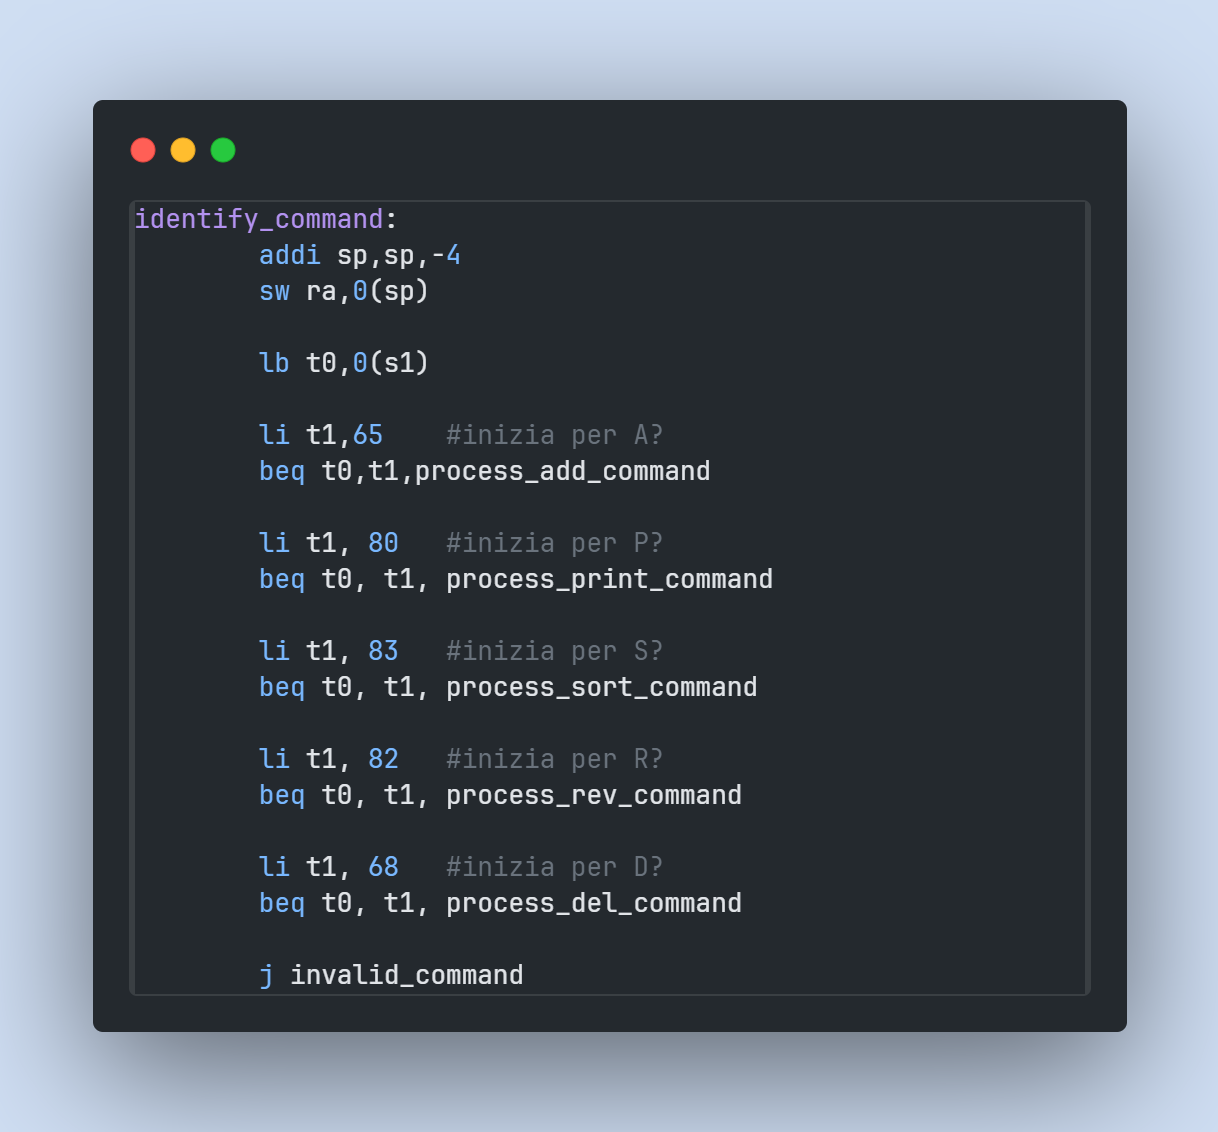
\includegraphics[width=0.40\linewidth]{img/identify_command.png}
                \label{fig:1b}
            }
            \label{fig1}
            \caption[]{}
        \end{figure}
        
       Se il controllo non viene trasferito, scorro la stringa (tramite \textit{find\_next\_command}), finché non trovo una tilde o un fine stringa, per poi ritornare nel loop principale e ricominciare la fase di identificazione comando. \\
       Altrimenti,la procedura \textit{process\_\textbf{x}\_command} trasferisce il controllo a \textit{verify\_\textbf{x}\_format} (dove \textbf{x} è il comando in questione).
       Se il comando è correttamente formattato e finisce con un terminatore valido (spazio o $\sim$) allora la verifica termina correttamente (cioé il metodo ritorna \textbf{1} in  \textit{a1})\footnote[1]{\textit{Il valore di ritorno della funzione di validazione sarà in a1 per evitare interferenze con comandi che accettano parametri nel registro \textit{a0} come ADD e DEL}} e lo eseguo tramite \textit{jump-and-link} alla rispettiva procedura.\\ Terminata l'operazione avanzo di un carattere.

    \section{verify\_\textbf{x}\_format}
    
    \begin{mdframed}
        \texttt{parametri:} nessuno \\
         \texttt{ritorno:}\textit{a1}  (\textcolor{ForestGreen}{1 - successo}, \textcolor{Red}{0 - fallimento})\\
         \texttt{cosa fa:} ritorna se il formato del comando \textbf{x} è valido o meno

    \end{mdframed}
    La funzione di verfica controlla sequenzialmente
    \begin{enumerate}
        \item se i caratteri successivi sono quelli propri del comando in questione
        \item se il comando ha un parametro ammissibile (cioé un carattere ASCII fra 32 e 125
        \item se il comando ha un terminatore valido (tramite \textit{verify\_command\_terminator} che skippa eventuali spazi e controlla la presenza di un terminatore tilde/fine stringa valido 
        
    \end{enumerate}
    In caso di successo carica in \textit{a1} il valore 1 e ritorna con successo.\\
    In caso contrario vuol dire che è stata richiamata la procedura \textit{invalid\_format} che carica in \textit{a1} il valore 0 e ritorna al chiamante.
    \newpage
    \chapter{Funzioni}
    \section{Premessa}
    Le varie funzioni sono state implementate modularmente e sono state realizzate in modo da mantenere il più possibile valido il principio di regolarità, cruciale nell'architettura RISC-V. Tutte le funzioni che necessitano di parametri (cioé \textit{ADD} e \textit{DEL} li accettano nel registro \textit{a0}, mentre tutte le funzioni che devono restituire dei valori li restituiscono in \textit{a1}. Inoltre tutte le procedure salvano all'inizio

    \section{Funzioni principali}
    \subsection{ADD}
    \begin{mdframed}
        \texttt{parametri:} in \textit{a0} carattere ASCII (sarà il DATA del nodo) \\
         \texttt{ritorno:} nessuno \\
         \texttt{cosa fa:} aggiunge un carattere ASCII alla lista concatenata
    \end{mdframed}
    Per effettuare la ADD di un nodo, devo per prima cosa individuare un indirizzo di memoria di 5 byte libero, pertanto richiamo la procedura \textit{find\_next\_free\_addr} descritta di seguito, tra le procedure di supporto. Individuato l'indirizzo della prossima locazione di memoria libera, salva nel primo byte (deputato al DATA) il carattere passato come parametro e successivamente mi allineo ai successivi 4 byte, nei quali salverò l'indirizzo del prossimo nodo, che sarà nullo in quanto il nodo successivo non esiste.\\
    \uline{A questo punto distiguiamo il caso della prima ADD della catena dal caso di ADD successivo.}
    \begin{itemize}
        \item[$\diamond$]nel caso della prima ADD: aggiorno le variabili globali \textit{HEAD\_PTR} e \textit{LAST\_PTR} con l'indirizzo della testa del nodo appena inserito
        \item [$\diamond$]nel caso di nodo successivo: aggiorno il \textit{PAHEAD} del nodo precedente con l'indirizzo del nodo attuale e \textit{LAST\_PTR} con con l'indirizzo del nodo corrente.
    \end{itemize}
    \newpage
    \subsection{DEL}
    \begin{mdframed}
        \texttt{parametri:} in \textit{a0} carattere ASCII (occorrenze da eliminare) \\
         \texttt{ritorno:} nessuno \\
         \texttt{cosa fa:} elimina \textbf{tutti} i nodi contenenti quel carattere
    \end{mdframed}
    Se la lista non è vuota, inizia controllando la testa e se va eliminata, aggiorno HEAD\_PTR con il \textit{PAHEAD} di quel nodo (rendo quindi il nodo successivo la nuova testa). Dopo di che diminuisco il counter dei nodi e controllo nuovamente se il nodo diventato testa va anch'esso eliminato. Se la lista diventa vuota, aggiorno anche il \textit{LAST\_PTR} e termino.\\
    Altrimenti, se la testa non va eliminata, scorro tutti gli altri nodi e per ognuno, controlla il carattere del nodo a lui seguente e se coincide con il carattere da eliminare aggiorna di conseguenza i \textit{PAHEAD} del nodo precedente e del nodo successivo; quando arrivo all'ultimo nodo della catena, aggiorna il \textit{LAST\_PTR}.
    
    \begin{figure}[H]
            \centering
            \includesvg[width=0.75\linewidth]{img/after-del.svg}
            \caption{Esempio di funzionamento di DEL}
            \label{fig}
    \end{figure}


    \subsection{PRINT}
    \begin{mdframed}
        \texttt{parametri:} nessuno \\
         \texttt{ritorno:} nessuno \\
         \texttt{cosa fa:} stampa ordinatamente tutti i nodi della catena
    \end{mdframed}

    La stampa è gestita ricorsivamente, a partire dalla testa tramite la procedura \textit{print\_recursive} (che accetta in \textit{a0} un indirizzo, la quale stampa, se la HEAD non è zero (a causa di lista vuota o raggiungimento dell'ultimo elemento) il carattere di un nodo. Dopo di che, richiama ricorsivamente sé stessa, ma dopo aver aver scorso al nodo successivo e passando in \textit{a0} l'indirizzo del nodo successivo.\\
    Per quanto concerne la gestione della memoria, ad ogni chiamata di \textit{print\_recursive} salvo nella stack sia il \textit{ra} come avviene usualmente e anche l'\textit{a0} che contiene l'indirizzo del nodo attuale (in totale salvo quindi 2 parole, cioé 8 bytes). Il salavataggio di \textit{a0} mi serve per poi riprenderlo dopo aver stampato uno spazio separatore (RIPES richiede per la stampa di un carattere di passare in \textit{a0} il carattere e in \textit{a7} il codice 1 per poi effettuare la \textit{ecall}).


    \subsection{SORT}{
  
    
        \begin{mdframed}
            \texttt{parametri:} nessuno \\
             \texttt{ritorno:} nessuno \\
             \texttt{cosa fa:} ordina tramite algoritmo bubble sort ricorsivo i vari nodi, sulla base delle regole di ordinamento prefissate
        \end{mdframed}

    La funzione di ordinamento implementa bubbleSort ricorsivo con flag di controllo di avvenuti scambi. Il problema principale nel fare ciò è quello di rispettare le regole custom di ordinamento, brevemente riassunte di seguito:

    \small
    \begin{itemize}
        \color{orange}\item una lettera maiuscola (ASCII da 65 a 90 compresi) viene sempre ritenuta maggiore di una minuscola
        \color{blue}\item una lettera minuscola (ASCII da 97 a 122 compresi) viene sempre ritenuta maggiore di un numero
        \color{magenta}\item un numero (ASCII da 48 a 57 compresi) viene sempre ritenuto maggiore di un carattere extra che implementiamo non sia una lettera funzione o numero
        \color{black}\item non si considerano accettabili caratteri extra con codice ASCII minore di 32 o maggiore di 125.
    \end{itemize}

    L'approccio adottato è quello di \textit{"categorizzare"} i vari caratteri ed effettuare per caratteri di tipo differente, confronti basati sulla categoria.\\
    Nel mio caso:
    \begin{mdframed}
        
    \begin{itemize}
    \label{categorie}
        \item[$\diamond$] \textcolor{orange}{maiuscola} $\rightarrow$ categoria 3
        \item[$\diamond$] \textcolor{blue}{maiuscola} $\rightarrow$ categoria 2
        \item[$\diamond$] \textcolor{magenta}{numero} $\rightarrow$ categoria 1
        \item[$\diamond$] \textcolor{black}{caratteri speciali} $\rightarrow$ categoria 0
        \item[$\diamond$] \textcolor{red} {carattere non valido} $\rightarrow$ categoria -1
    \end{itemize}
    
    \end{mdframed}
    Tale categorizzazione viene effettuata dalla procedura \textit{get\_category} che prende in \textit{a0} il carattere da valutare e restituisce in \textit{a1} il numero della categoria.

    Il resto del bubble sort viene gestito in maniera abbastanza semplice, tramite due cicli annidati. Il più esterno si occupa di gestire il caso in cui abbia finito la ricorsione e di resettare il flag di scambio avvenuto per ogni iterazione.\\
    Il più interno, dopo aver salvato nella stack\footnote[1]{Ho decrementato lo stack pointer di 8 sebbene i byte che utilizzi siano effettivamente 7 (4 per contenere un indirizzo, e poi 3 per contenere il DATA del nodo corrente, del successivo e il contatore dei nodi ancora da processare) per evitare problemi di allineamento} controllato se è arrivato all'ultimo nodo, ottiene le categorie del carattere corrente e quella del successivo e sulla base dei valori restituiti valuta se effettuare o meno lo swap fra i DATA dei due nodi.\footnote[2]{Non è necessario agire sui puntatori, ma semplicemente sulle informazioni contenute}
    Lo swap avviene appoggiandomi alla stack piuttosto che a registri temporanei e infine mettendo a \textit{true} il flag di scambio avvenuto. \footnote[3]{L'uso di un flag mi permette di evitare, nel caso di catena già ordinato, di effettuare scambi superflui}
    }
    
    \subsection{REV}
    \begin{mdframed}
            \texttt{parametri:} nessuno \\
             \texttt{ritorno:} nessuno \\
             \texttt{cosa fa:} inverte la lista concatenata
        \end{mdframed}
    


    \section{Funzioni di supporto}
    Le funzioni principali \textit{ADD} e \textit{SORT} all'interno del loro corpo fanno riferimento a delle procedure di supporto: in particolare \textit{ADD} usa \textit{find\_next\_free\_addr} per individuare 5 byte liberi in memoria per l'inserimento di un nodo, mentre \textit{SORT} utilizza \textit{get\_category} per determinare la categoria del carattere.

    \subsection{\textit{find\_next\_free\_addr}}

    \begin{mdframed}
            \texttt{parametri:} nessuno \\
             \texttt{ritorno:} indirizzo di memoria (word) in a1\\
             \texttt{cosa fa:} restituisce un indirizzo all'inizio di una porzione di 5 byte liberi
        \end{mdframed}

        La funzione in sé non è particolarmente complicata: scansiona sequenzialmente ogni byte a partire da un indirizzo base fisso (\textit{0x20000000})\footnote[1]{Ho scelto questo indirizzo di partenza per evitare del tutto conflitti con \textit{listInput}molto lunghi} finché non ne individua 5 consecutivi liberi, ritornando poi l'indirizzo della testa e aggiornando la variabile globale \textit{s5}che contiene la il byte immediatamente successivo ai 5 appena individuati, funzionale per scansioni successive. 
        
    \subsection{\textit{get\_category}}

    \begin{mdframed}
            \texttt{parametri:} carattere (1 byte) in a0 \\
             \texttt{ritorno:} categoria (intero) in a1 \\
             \texttt{cosa fa:} restituisce la categoria di un carattere \small(si veda \ref{categorie})
        \end{mdframed}

        La procedura è in realtà abbastanza semplice: preso un carattere, controlla innanzitutto la sua ammissibilità (cioé se è un ASCII tra 32 e 125), poi se è una lettera maiuscola (ASCII fra 65 e 90), maiuscola $\ldots$ \\


    \chapter{Ulteriori osservazioni e conclusioni}
    \chapter{}
    
    
    
    
\end{document}